\chapter{Luogo delle radici}
\section{Metodo di risoluzione}
Il metodo consiste nel dividere lo svolgimento del problema in microaree.
\begin{enumerate}
	\item \emph{Mappa poli-zeri}: ovvero le radici del denominatore (poli)
		convenzionalmente segnati con una croce, mentre le radici del
		numeratore (zeri) segnati con un cerchio.
	\item \emph{Punti sull'asse reale}: si evidenzia la parte di asse reale
		che si sviluppa a sinistra di un polo/zero, con a destra un numero
		dispari di poli/zeri.
	\item \emph{Determinare gli asintoti}: si calcola il centroide e l'angolo
		di inclinazione degli asintoti con le seguenti formule:
		\begin{align*}
			& \sigma_a = \frac{\sum_{i} p_i - \sum_{i} z_i}{n-m} \\
			& \theta_a = \frac{(2\nu+1)\pi}{n-m} \quad \text{con } \nu = \bigl\{ 0,\dots,n-m-1 \bigr\}
		\end{align*}
		con \(n\) e \(m\) rispettivamente grado del denominatore e grado del numeratore.
	\item \emph{Angoli di partenza e di arrivo per i punti di emergenza/confluenza}
	\item \emph{Intersezioni con l'asse immaginario e punti doppi}
		per i punti doppi si calcolano le radici di \(G^\prime(s) = 0\).
		Se però si ha un grado eccessivamente elevato, si può ricorrere
		alla \emph{tabella di taratura}, ponendo valori di \(s\) appartenenti
		al luogo delle radici e ottenere un valore \(k\) tale che
		\[
			k = -\frac{1}{G(s)}
		\]
		Per un punto di emergenza ci si deve aspettare un massimo locale,
		mentre per un punto di confluenza un minimo locale.
	\item \emph{Studio della stabilità al variare di \(k\)}: con valori
		di \(k\) \emph{critici} (ovvero noti), si può intuire
		dal grafico la stabilità del sistema seguendo i rami orientati;
		se si dovesse studiare la stabilità per \(k \in \mathbb{R}\) è
		meglio ricorrere al \emph{criterio di Routh}.
\end{enumerate}

\begin{nota}
Durante gli esercizi è possibile che il \(k\) venga sottinteso dalla traccia,
avendo quindi solo \(G(s)\).
\end{nota}

\begin{esercizio}
Sia data la seguente funzione di trasferimento con parametro \(k\)
\[
	kG(s) = k \frac{s+1}{s \bigl( s+2 \bigr)}
\]
Determinare il luogo delle radici al variare di \(k > 0\).

\paragraph{Soluzione}

\begin{figure}[ht]
	\centering
	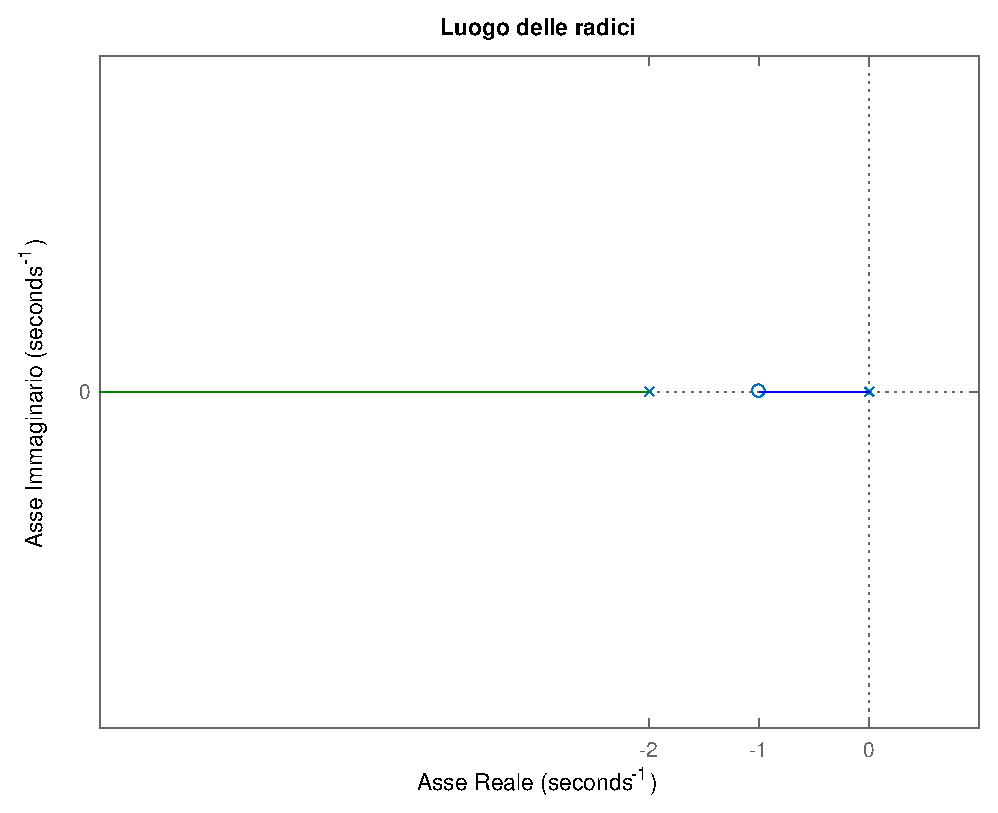
\includegraphics[scale=.6]{mod1/assets/rl_ex31}
\end{figure}

Determino centroide e angolo di inclinazione degli asintoti:
\[
	\sigma_a = \frac{0 -2 +1}{1} = -1
	\qquad
	\theta_a = \frac{(2\nu+1)\pi}{n-m} = \pi
\]

L'esercizio non richiede altro lavoro perché non presenta punti doppi, di
intersezione con l'asse immaginario, etc.

Studio la stabilità:
\[\begin{cases}
	k = 0 & \text{sistema \emph{semplicemente stabile}} \\
	k > 0 & \text{sistema \emph{asintoticamente stabile}} \\
\end{cases}\]
\end{esercizio}

\begin{esercizio}
Sia data la seguente funzione di trasferimento:
\[
	G(s) = \frac{s+1}{s^2}
\]
Determinare il luogo delle radici al variare di \(k > 0\).

\paragraph{Soluzione}

\begin{figure}[ht]
	\centering
	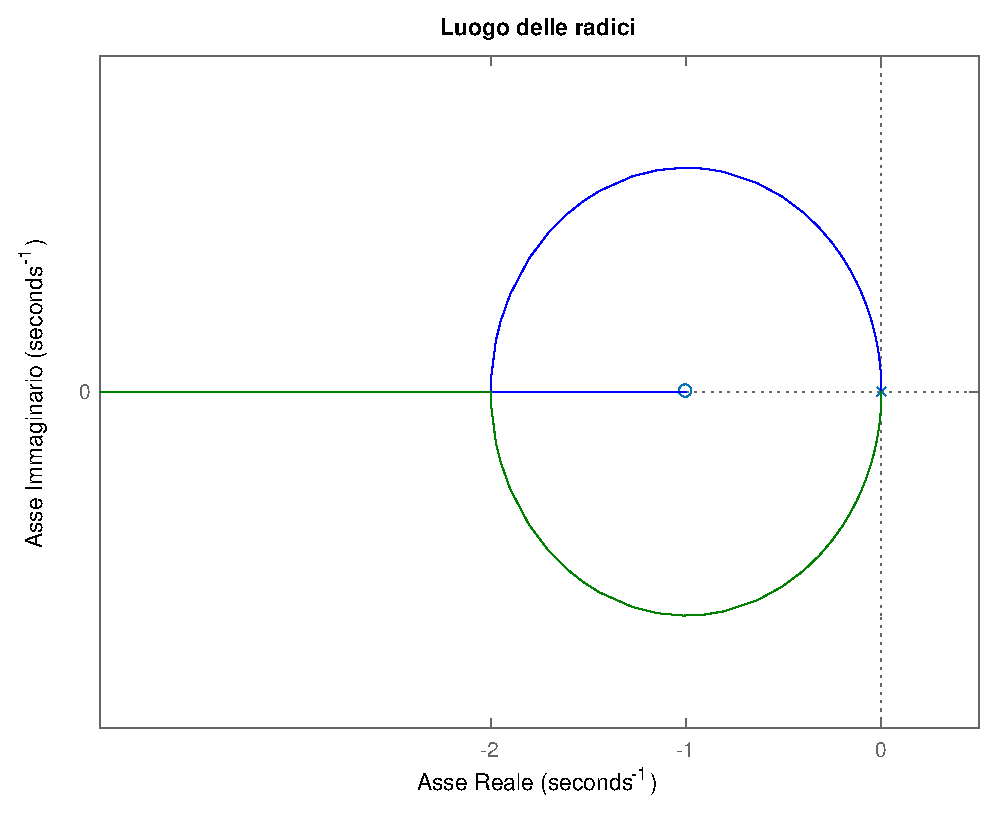
\includegraphics[scale=.6]{mod1/assets/rl_ex32}
\end{figure}

\begin{itemize}
	\item Poli: \(\bigl\{ 0\,[\times 2] \bigr\}\)
	\item Zeri: \(\bigl\{ -1 \bigr\}\)
	\item Asintoti: \(\sigma_a = \frac{0+1}{1} = 1\), \(\theta_a = \pi\)
	\item Gli angoli di arrivo e di partenza sono entrambi di
		\(\pm \frac{\pi}{2}\), questo perché non sono punti complessi e
		coniugati.
	\item Posizione del punto di confluenza:
		\[
			G^\prime(s) = \frac{s^2 -2s(s+1)}{\cancel{s^2}} = 0
			\rightarrow s(s+2) = 0
			\implies s= \begin{cases} 0 \\ \bm{-2} \end{cases}
		\]
	\item Stabilità:
		\[\begin{cases}
			\text{Se } k = 0\colon & \text{sistema \emph{semplicemente stabile}} \\
			\text{Se } k > 0\colon & \text{sistema \emph{asintoticamente stabile}}
		\end{cases}\]
\end{itemize}
\end{esercizio}

\begin{esercizio}
Sia data la seguente funzione di trasferimento
\[
	G(s) = \frac{1}{s(s+1)(s+5)}
\]
Determinare il luogo delle radici al variare di \(k>0\).

\paragraph{Soluzione}

\begin{figure}[ht]
	\centering
	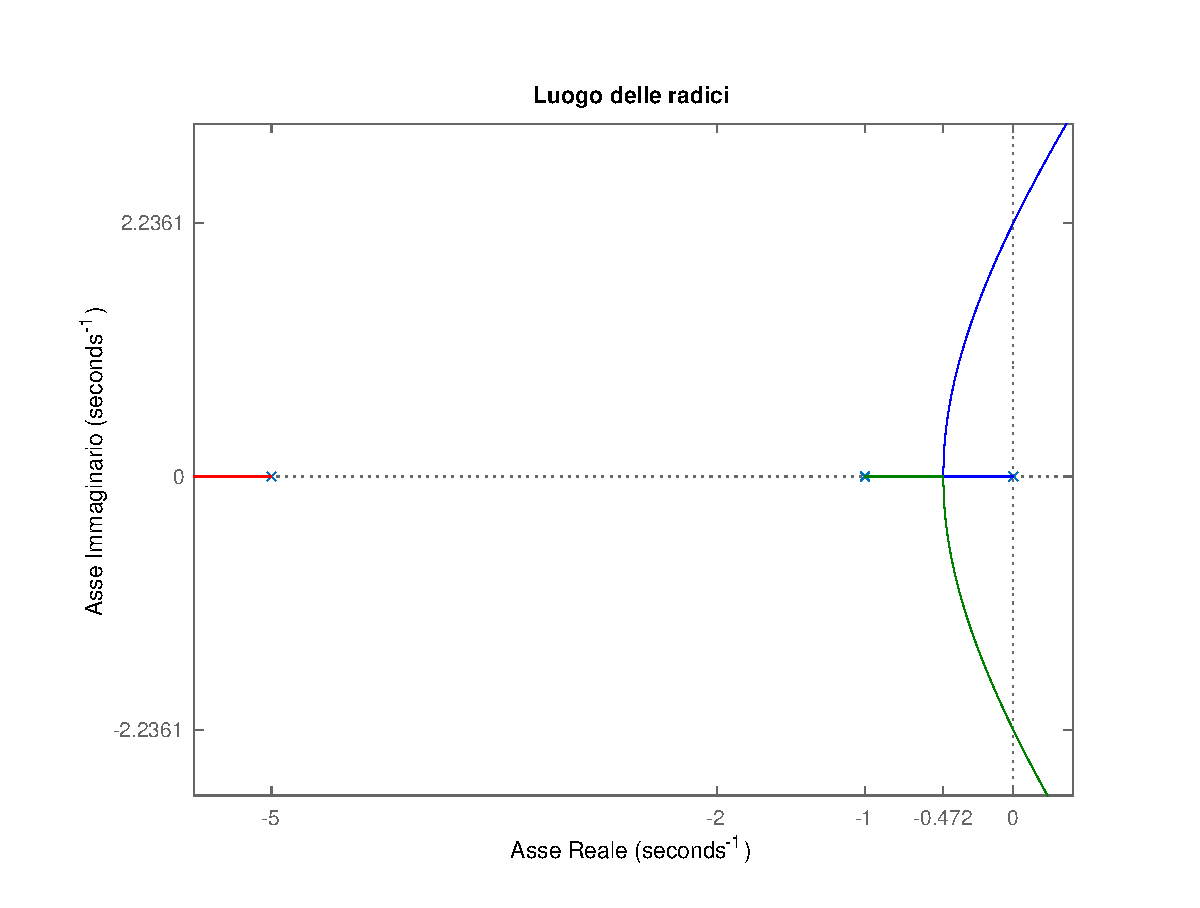
\includegraphics[scale=.6]{mod1/assets/rl_ex33}
\end{figure}

\begin{itemize}
	\item \emph{Punti di singolarità}:
		\begin{itemize}
			\item poli: \(\bigl\{ -5, -1, 0 \bigr\}\)
		\end{itemize}
	\item \emph{Asintoti}:
		\begin{align*}
			& \sigma_a = \frac{0-1-5}{3} = -2 \\
			& \theta_a = \frac{\Bigl( 2 \cdot \bigl\{ 0, \dots, 2 \bigr\} +1 \Bigr) \pi}{3} = \bigl\{ \frac{\pi}{3}, \pi, \frac{5}{3}\pi \bigr\}
		\end{align*}
	\item \emph{Punto doppio di emergenza}:
		\[
			G^\prime (s) = 0 \rightarrow -3s^2 -12s -5=0 \rightarrow s_{1,2} = \frac{-6\pm\sqrt{21}}{3} = \begin{cases} \bm{-0.472} \\ -3.527 \end{cases}
		\]
		Si sceglie il primo perché è il valore che appartiene al luogo delle radici.
	\item \emph{Punti di intersezione con l'asse immaginario}:
		applico il criterio di Routh per \(P(s) = s^3 +6s +5s +k\):
		\[\begin{array}{r|rr}
			s^3      & 1 & 5 \\
			\bm{s^2} & 6 & k \\
			s^1      & \bm{30-k} \\
			s^0      & k
		\end{array}\]
		\[
			k = 30 \rightarrow 6s^2+30 = 0 \rightarrow s = \pm \jmath \sqrt{5}
		\]
	\item \emph{Stabilità}:
		\[\begin{cases}
			\text{Se } k = 0\colon & \text{sistema \emph{semplicemente stabile}} \\
			\text{Se } 0 < k < 30\colon & \text{sistema \emph{asintoticamente stabile}} \\
			\text{Se } k = 30\colon & \text{sistema \emph{semplicemente stabile}} \\
			\text{Se } k > 30\colon & \text{sistema \emph{instabile} con 2 poli instabili}
		\end{cases}\]
\end{itemize}
\end{esercizio}

\begin{esercizio}
Sia data la seguente funzione di trasferimento:
\[
	G(s) = \frac{(s+1.5)(s+4)}{s(s+1)(s+2.5)}
\]
Determinare il luogo delle radici per \(k>0\).

\paragraph{Soluzione}

\begin{figure}[ht]
	\centering
	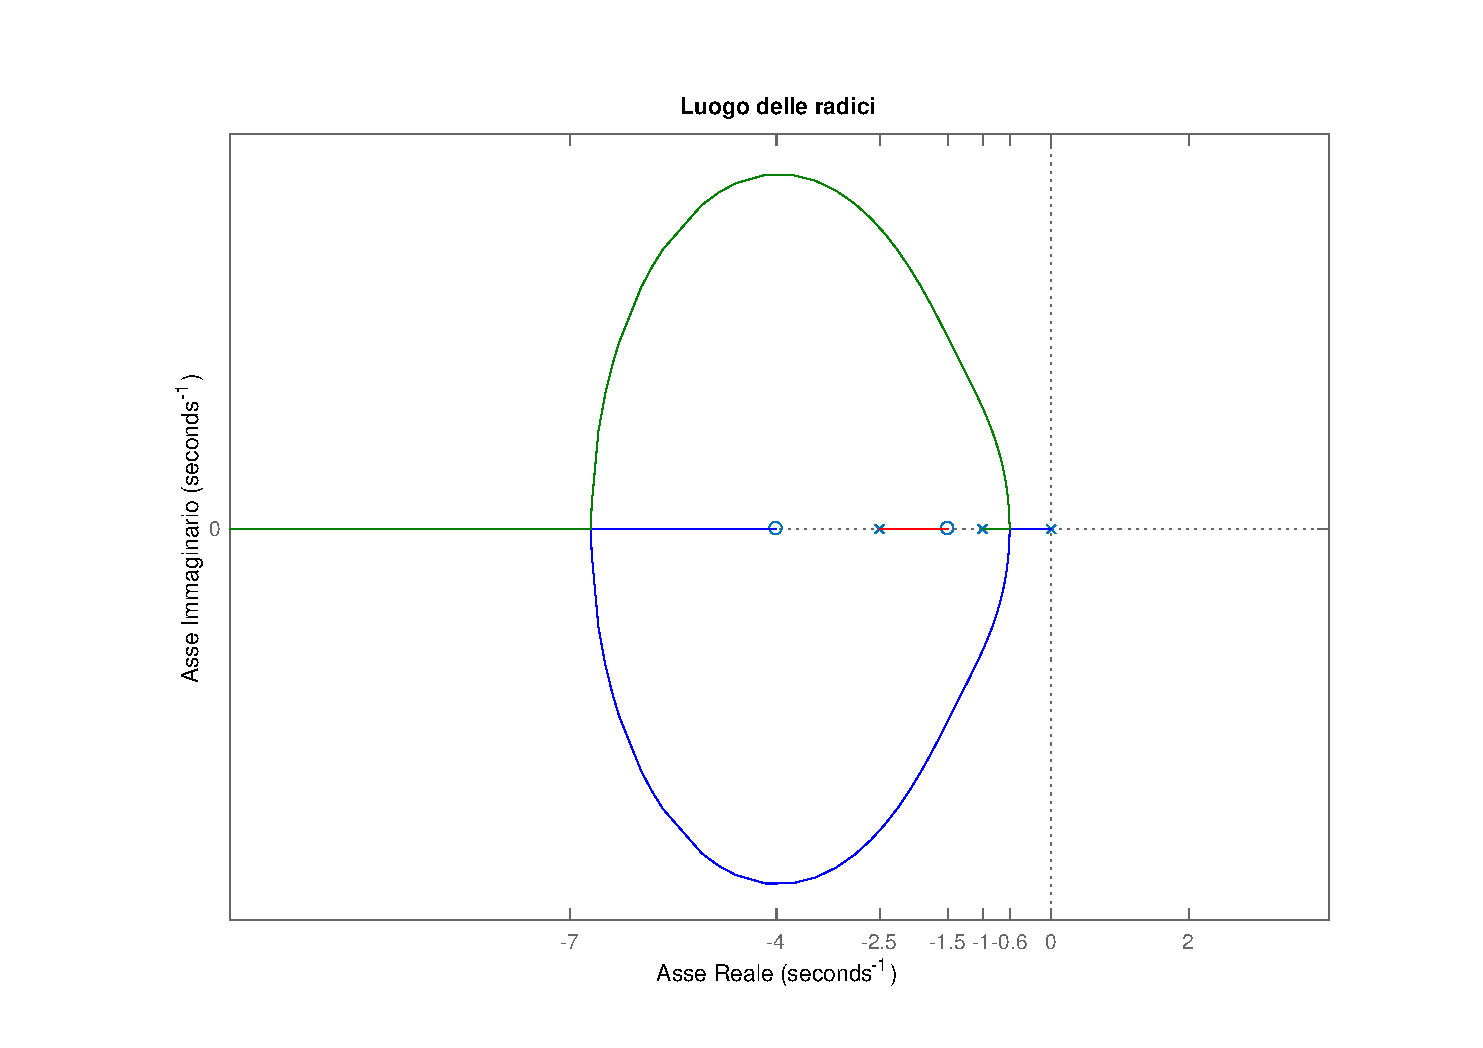
\includegraphics[scale=.6]{mod1/assets/rl_ex34}
\end{figure}

\begin{itemize}
	\item \emph{Punti di singolarità}:
		\begin{itemize}
			\item zeri: \(\bigl\{ -4, -1.5 \bigr\}\)
			\item poli: \(\bigl\{ -2.5, -1, 0 \bigr\}\)
		\end{itemize}
	\item \emph{Asintoti}:
		\begin{align*}
			& \sigma_a = \frac{0-1-2.5+1.5+4}{1} = 2 \\
			& \theta_a = \frac{\Bigl( 2 \cdot \bigl\{0\bigr\} +1 \Bigl)}{1} = \pi
		\end{align*}
	\item \emph{Punto doppio di emergenza}:
		lo ricavo con la tabella di taratura
		\[\begin{array}{rr}
			\toprule
			s & k \\
			\midrule
			-0.2 & 0.074 \\
			-0.4 & 0.127 \\
			\bm{-0.6} & \bm{0.149} \\
			-0.8 & 0.12 \\
			\bottomrule
		\end{array}\]
		Per \(s = -0.6\) si ha il massimo locale, ovvero il punto più
		approssimato al punto di emergenza.
	\item \emph{Punto doppio di confluenza}:
		\[\begin{array}{rr}
			\toprule
			s & k \\
			\midrule
			-5 & 14.286 \\
			-6 & 11.667 \\
			\bm{-7} & \bm{11.454} \\
			-8 & 11.846 \\
			\bottomrule
		\end{array}\]
		Per \(s = -7\) si ha il minimo locale, ovvero il più approssimato
		al punto di confluenza.
	\item \emph{Stabilità}:
		\[\begin{cases}
			k = 0\colon & \text{sistema \emph{semplicemente stabile}} \\
			k > 0\colon & \text{sistema \emph{asintoticamente stabile}}
		\end{cases}\]
\end{itemize}
\end{esercizio}

\begin{esercizio}
Sia data la seguente funzione di trasferimento:
\[
	G(s) = \frac{s+1}{s^2 (s+4)}
\]
Determinare il luogo delle radici per \(k>0\).

\paragraph{Soluzione}

\begin{figure}[ht]
	\centering
	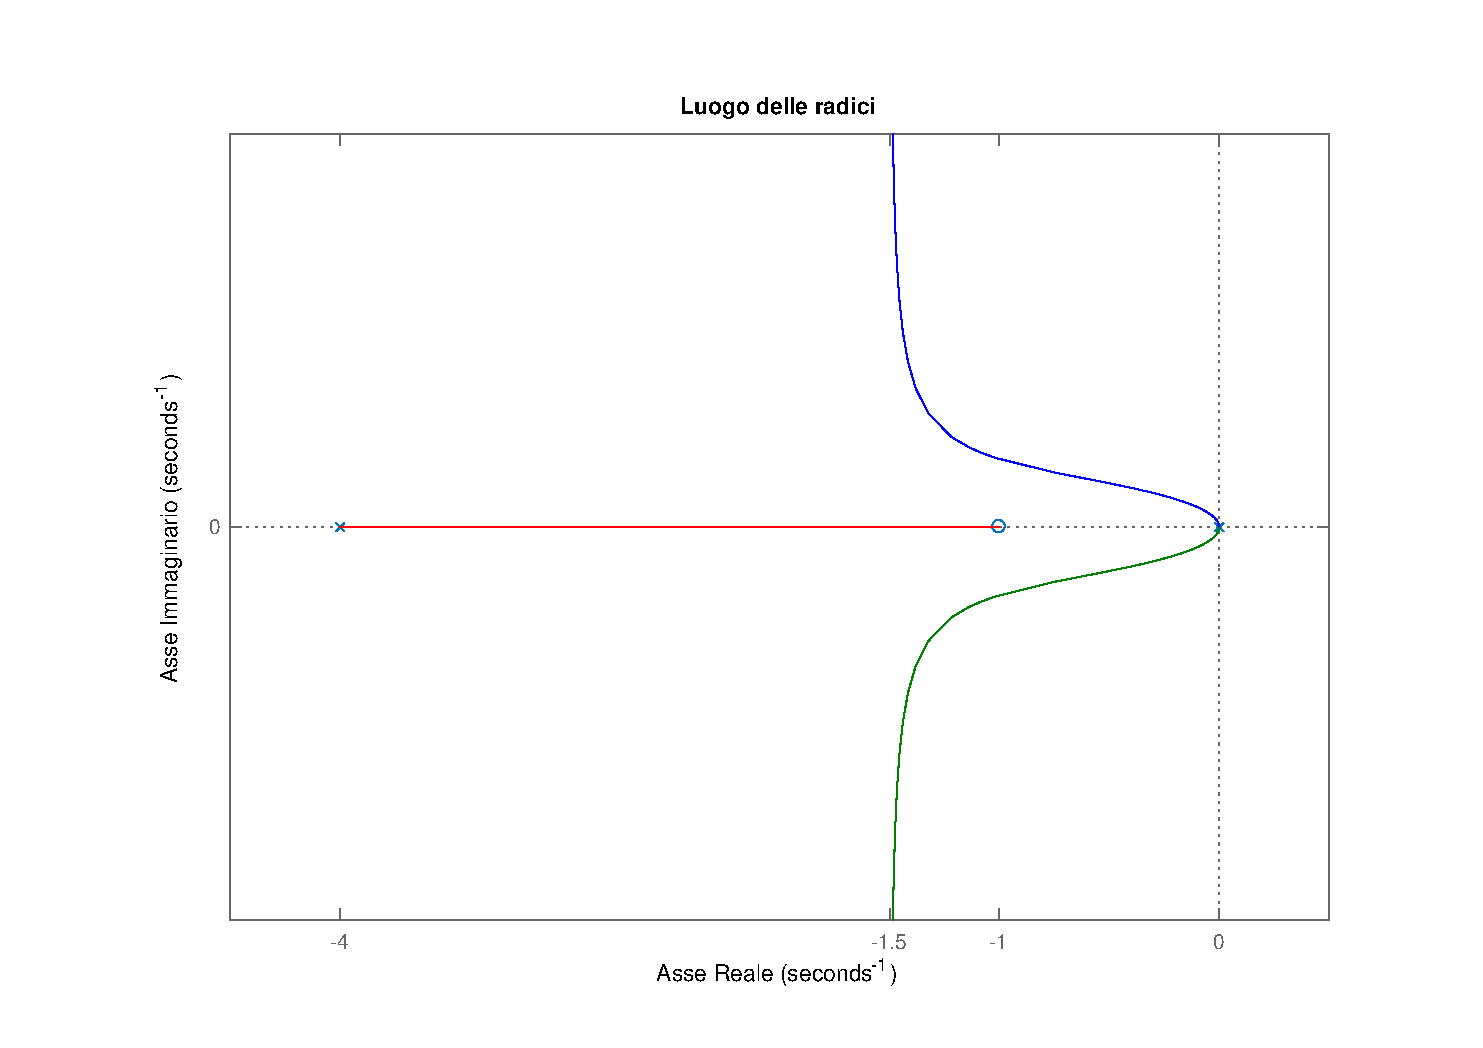
\includegraphics[scale=.6]{mod1/assets/rl_ex35}
\end{figure}

\begin{itemize}
	\item \emph{Punti di singolarità}:
		\begin{itemize}
			\item poli: \(\bigl\{ -4, 0\,[\times 2] \bigr\}\)
			\item zeri: \(\bigl\{ -1 \bigr\}\)
		\end{itemize}
	\item \emph{Asintoti}:
		\begin{align*}
			& \sigma_a = \frac{0-4+1}{2} = -\frac{3}{2} \\
			& \theta_a = \frac{\Bigl( 2 \cdot \bigl\{ 0,1 \bigr\} \pi \Bigr) \pi}{2} = \Bigl\{ \frac{\pi}{2}, \frac{3}{2}\pi \Bigr\}
		\end{align*}
	\item \emph{Angoli di partenza dei rami}: \(\frac{\pi}{2}\)
\end{itemize}
\end{esercizio}